\documentclass[../rapport_MVEX01-11-05]{subfiles}
\begin{document}

\subsection{Klassificering av gester med hjälp av \knn}

Den största andelen korrekt klassificerade gester vi lyckades uppnå var 91,5\%.
Denna procent uppnåddes då samtliga gester var inkluderade, antalet aktiverade
egenskaper var 10 och värdet på $k$ i kNN-metoden var 7. Egenskaperna som
användes var det första, andra, tredje och sjunde Hu-momentet, centroidens
position i den inneslutande lådan, fyrkantighet, soliditet, excentricitet,
konvexitet och utsträckning. Följande plot visar hur andelen korrekta
klassficeringar beror på antalet aktiverade egenskaper och värdet på $k$:

(PLOT)

Det framgår tydligt att antalet aktiverade egenskaper har stor inverkan på
resultatet då man använder sig av färre än 5st. Därefter planar procenttalet ut
för att återigen stiga då fler än 10 egenskaper används. Andelen korrekta
klassificeringar ökar också i takt med att $k$ ökar från 1 till 7, för att sedan
bidra negativt då värdet ökar från 7 till 13. Med det optimala valet av
egenskaper och $k$ blev prestandan för respektive gest

\begin{table}
	  \centering
		\label{tab:tolkningsmatris}
		\caption{SKRIV MIG!}
    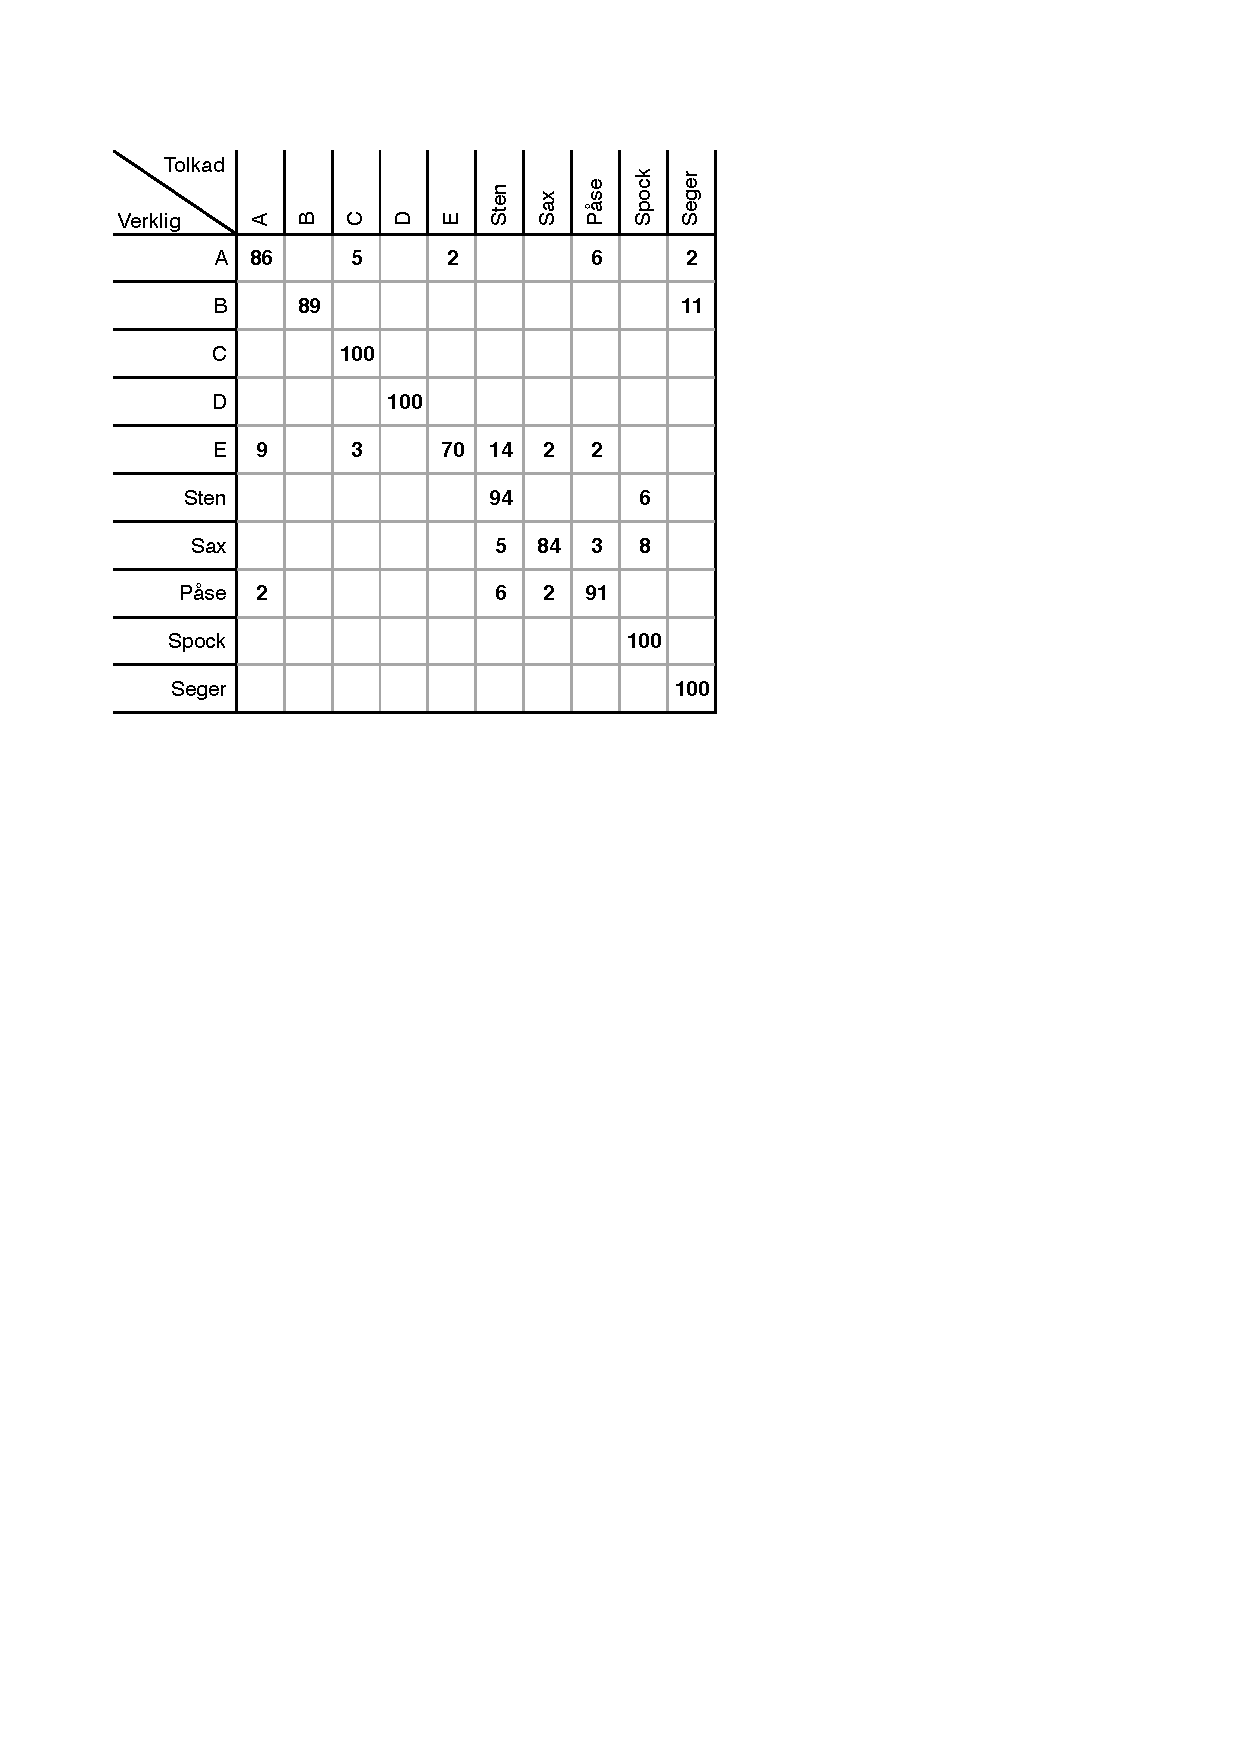
\includegraphics[trim=0 0 0 2.5cm]{bilder/tolkningsmatris.pdf}
		%\begin{tabular}{l|cccccccccc}
		%\backslashbox{Verklig}{Tolkad} & a & b & c & d & e & Sten & Sax & PÃ¥se & Spock & Seger\\
		%\toprule
		%a & 86 &  & 5 &  & 2 &  &  & 6 &  & 2 \\ 
		%b &  & 89 &  &  &  &  &  &  &  & 11 \\ 
		%c & &  & 100 &  &  &  &  &  &  &  \\ 
		%d &  &  &  & 100 &  &  &  &  &  &  \\ 
		%e & 9 &  & 3 &  & 70 & 14 & 2 & 2 &  &  \\ 
		%Sten & &  &  &  &  & 94 &  &  & 6 &  \\ 
		%Sax & &  &  &  &  & 5 & 84 & 3 & 8 &  \\ 
		%PÃ¥se & 2 &  &  &  &  & 6 & 2 & 91 &  &  \\ 
		%Spock &  &  &  &  &  &  &  &  & 100 &  \\ 
		%Seger & &  &  &  &  &  &  &  &  & 100 \\  
		%\end{tabular}
\end{table}

(Inkludera resultat där problemgester är borttagna?)

(i ordning: det tredje Hu-momentet, det andra Hu-momentet, centroidens
y-position i den inneslutande lådan, fyrkantighet, soliditet, excentricitet,
konvexitet, första Hu-momentet, utsträckning och det sjunde Hu-momentet.) 

%\notes{Jag vill ha den som \LaTeX{} men inte som en ''ful'' tabell. Det verkar
%finnas ett paket \texttt{slashbox} som gör den sneda biten, i komination med
%typ \texttt{colortbl} kan det bli hyfsat okej. Men riktiga tabeller ska vi nog
%använda \texttt{booktabs till}.}

\end{document}
